\chapter{Projektplanung}
\label{chap:projektablauf}

	In diesem Kapitel wird der Begriff Projekt abgegrenzt, sowie auf die unterschiedlichen Projektphasen eingegangen. Diesbezüglich dient dieses Kapitel zur Klärung der Frage: \ersteUnterfrage

\section{Projekt}

	Die Ursache für die Entstehung eines Projektes, liegt primär in einem ungedeckter Bedarf. Für die Erfüllung eines solchen Bedarfs fallen mehrere unterschiedliche Aufgaben, die von Menschen aus unterschiedlichen Bereichen, Abteilungen, Unternehmen oder in einigen Fällen Ländern erfüllt werden, an. Jeder dieser Mitarbeiter ist ein essentieller Bestandteil des Projektfortschritts. Die zu erfüllenden Aufgaben werden Kategorisiert, sowie in einen Zeitlichen Zusammenhand gesetzt.\cite[4]{Wysocki_2019_Projekt}
	
	Diese aneinander gereihten Aufgaben werden Teilprozesse genannt und tragen entscheidend zu der Fertigstellung eines größeren Vorhabens, welches Prozess genannt wird, bei. Madauss beschreibt ein Projekt als \enquote{\textit{Vorhaben mit definiertem Anfang und Abschluss, das durch die Merkmale zeitlicher Befristung, Einmaligkeit, Komplexität und Neuartigkeit gekennzeichnet ist.}}\cite[4]{Madauss2020} Die ISO Norm bezeichnet diese Art von Vorhaben als eine \enquote{Gruppe von Prozessen}\cite[11]{ISO10006_2019}, welche zusammen ein ganzes ergeben. Somit ist ein Projekt durch die folgenden Punkte gekennzeichnet: 
	
	\begin{itemize}
		\item Einzigartigkeit 
		\item Komplexität
		\item Zusammenhängende Aktivitäten
		\item Bestehend aus mehreren Teilprozessen
		\item Zeitliche Befristung 
		\item Einem gemeinsamen Ziel
		\item Einem bestimmten Budget
	\end{itemize}
	
	Unter der Berücksichtigung der oben erwähnten Punkte, lässt sich ein Projekt also als ein einmaliges Vorhaben beschreiben, welches ein bestimmtes Ziel verfolgt, eine gewisse Komplexität mit sich bringt und über ein vorgegebenes Budget verfügt. \cite[4-7]{Wysocki_2019_Projekt}
	Die Erreichung wird durch Projektphasen gewährleistet, die neben der Überwachung des Fortschritts auch die noch zu erreichenden Teilziele abdecken. 
	
\section{Lebenszyklus}
	
	Projekte können Abhängig von der Größe, sowie der Branche in welcher sie durchgeführt werden, mehrere Wochen oder Jahre dauern. So kann sich Beispielsweise die Entwicklung einer Software über mehrere Jahrzehnte ziehen. Die Bearbeitung eines solchen Vorhabens unterteilt sich grundsätzlich in logisch aufeinander folgende Phasen, die das Projektmanagements von der Definition der Zielvorgabe bis zum Abschluss begleiten. Sie stellen außerdem das Grundkonzept des Projektmanagements dar.\autocite[107-110]{madauss2019} Jede Phase steht hierbei für einen in sich geschlossenen Teil des Projektes, der über die Definition der Hauptaufgabe in der jeweiligen Phase verfügt, sowie eine Auskunft über das genaue vorgehen in der Phase gibt. Eine Phase beschreibt außerdem durch die Definition von Meilensteinen genau welche Aufgaben nach Abschluss einer Phase erledigt sein müssen. Bei der Abnahme dieser Phase dienen die Meilensteine als Abnahmekriterien anhand dessen der Fortschritt festgestellt werden kann.\autocite[16]{Meyer2020}
	
	Zusammengefasst werden diese Phasen unter dem Begriff \ac{LZ} eines Projektes verstanden. Ziel des Lebenszyklus ist es, ein klares Vorgehen im Projekt zu schaffen, wodurch ein nachvollziehbarer Projektplan entstehen kann und somit auch eine Baseline. Als baseline bezeichnet man einen Projektplan, der den Grundstein eines Projektes darstellt. Je nach Branche kann sich der \acs{LZ} eines Projektes unterscheiden.\autocite[14]{Meyer2020} In der IT-Branche beispielsweise gibt es auch Branchenintern einige geringfügige Unterschiede. So spricht die ISO-Norm von fünf Projektphasen \autocite[11]{DIN69901-2}, während das amerikanische Project Management Institute lediglich von vier Phasen spricht. Die PRINCE2 geht einen schritt weiter und definiert lediglich zwischen zwei Abschnitten, nämlich des Initiierung und dem Ende. Es lässt gewollt Spielraum für die mittleren Phasen übrig, da die sich je nach zu erbringender Leistung unterscheiden\autocite[15]{Meyer2020}. Die Abbildung \ref{img:phasen} veranschaulicht die unterschiedlichen Herangehensweisen der definierten Standards. 
	
	\begin{figure}[h]
		\centering
		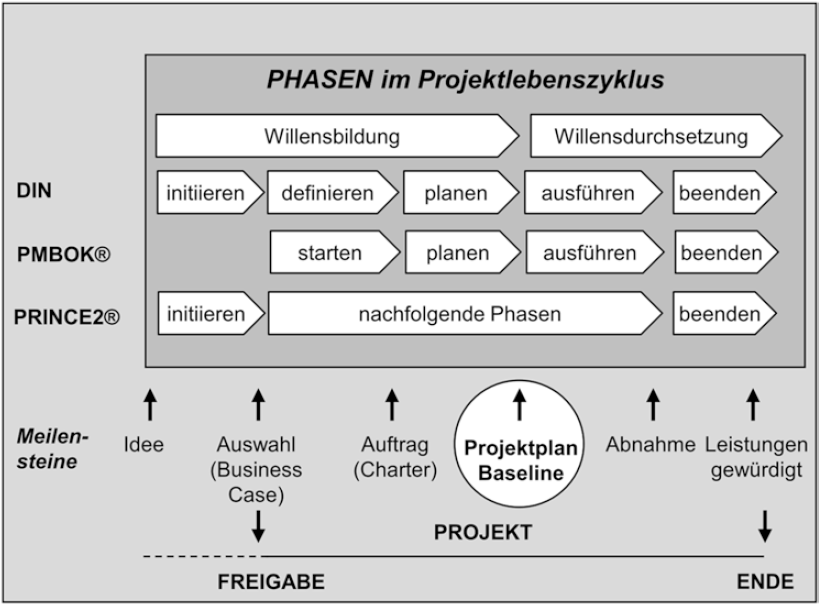
\includegraphics[width=15cm]{img/Projektlebenszyklus.png}
		\caption{Phasen der unterschiedlichen Normen\cite[15]{Meyer2020}}
		\label{img:phasen}
	\end{figure}

	Jede einzelne Phase übernimmt somit einen eigenen Bereich eines Projektes. Die Bereiche einer jeden Phase hängen von den Ergebnissen der vorherigen Phase ab\autocite[16]{Meyer2020}. Im folgenden werden die Phasen beschrieben: 
	
	\begin{enumerate}
		\item Initiierungsphase	
			\subitem Am Ende dieser Phase wird entschieden ob eine Projektidee zu einem realen Projekt wir, oder ob sie verworfen wird. Dies kann durch unterschiedliche Analysen untersucht werden, die jedoch nicht Teil dieser Arbeit sind.
			
		\item Definitionsphase
			\subitem In dieser Phase wird die Idee Konkretisiert, sowie geplant. Somit müssen die unterschiedlichen Stakeholder eingeweiht werden. Die Projektleitung muss aufgestellt werden. 
		\item Planungsphase
			\subitem In der Planungsphase erstellt das Projektteam bzw. der Projektleiter Pläne für die Durchführung des Vorhabens. Die primär berücksichtigten Faktoren bei der Planung sind Kosten, Qualität und Zeit. Der Projektleiter erstellt einen Projektstrukturplan, der das weitere Vorgehen eines Projektes bestimmen soll. 
		\item Umsetzphase
			\subitem In dieser Phase wird die hauptsächliche Leistung erbracht. Der Projektmanager ist hier primär mit der Überwachung und Steuerung des Projektes beschäftigt. 
		\item Abschlussphase
			\subitem Mit dieser Phase wird der Abschluss eines Projektes eingeläutet. Hier wird sowohl die erzielte Leistung als auch die Dokumentationen übergeben. Des weiteren werden Lessons-Learned aus dem Projekt gezogen sowie die Ressourcen zurück zu deren ursprünglichen Aufgaben zurückgeführt. 
						
	\end{enumerate}

	Diese Aufteilung eines Projektes in einzelne Projektphasen, gewährleistet nicht nur mehr  Kontrolle über die einzelnen Aktivitäten im Projekt, sondern ermöglicht es auch eine genauere Planung im Projekt durchzuführen. Durch eben diese Kontrolle können die Qualität, Kosten, Termine sowie Leistungsergebnisse im falle einer Abweichung frühzeitig identifiziert sowie korrigiert werden.\cite[57]{Känel_2020_Projektphasen}
	
	
\section{Projektphasenmodelle}
\label{sec:phasenmodell}

	Ein Phasenmodell wird folgendermaßen Definiert:
	
	\begin{quote}
		\enquote{\textit{Unter einem \textbf{Phasenmodell} ist im Rahmen des Projektmanagements eine weitgehend
		standardisierte Darstellung der Gliederung eines typischen Projektablaufs
		in sachliche und zeitliche Abschnitte zu verstehen.
		Diese Abschnitte müssen sich eindeutig bezeichnen lassen und dienen vor allem
		der Orientierung und Standortbestimmung im jeweiligen Projektablauf.}}\autocite[57]{Känel_2020_Projektphasen}
	\end{quote}
	
	Laut Känel stellen Phasenmodelle somit einen Rahmen dar, der einen Projektmanager bei der Planung und Kontrolle unterstützt. Die zu der Orientierung dienenden Rahmenwerke gibt es in unterschiedlichen Ausprägungen. Bei der Betrachtung solcher Modelle im Zusammenhang mit digitalem Projektmanagement lassen sich Grundsätzlich drei Ansätze unterscheiden. Das klassische Vorgehen im Projektmanagement, bei diesem Ansatz wird davon ausgegangen, dass ein Projekt von dem \enquote{Anfang} bis zum \enquote{Abschluss} durchgeplant werden kann. Somit werden die einzelnen Phasen möglichst genau vorausgeplant. Wodurch die einzelnen Phasen nach dem Plan sequentiell abgearbeitet. Ein typisches Vorgehensmodell für diesen Ansatz ist das \enquote{Wasserfallmodell} oder auch das \enquote{V-Modell}\autocite[Kap. 2]{Vivenzio2013}. Die Abbildung \ref{img:wasserfall} zeigt die typischen Phasen des Wasserfallmodells 

	\begin{figure}
		\begin{minipage}[b]{.4\linewidth} % [b] => Ausrichtung an \caption
			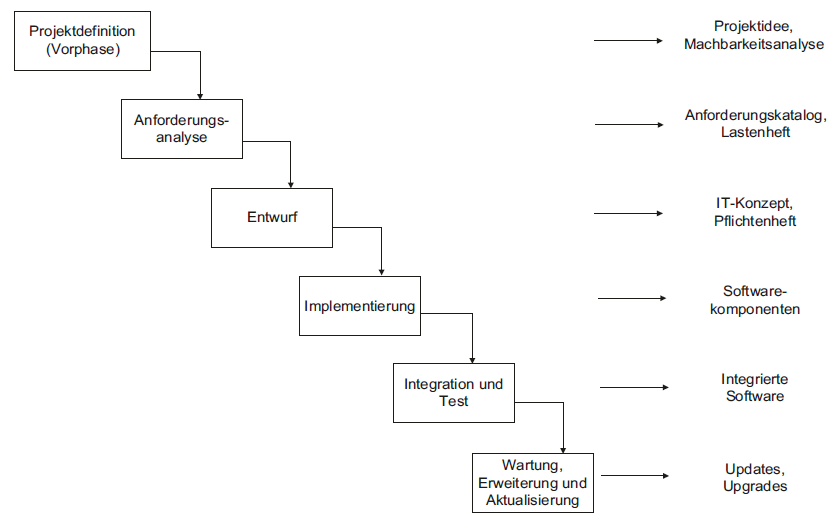
\includegraphics[width=8cm]{img/wasserfallmodell.png}
			\caption{klassisches Vorgehen: Wasserfallmodell \autocite[353]{Alpar2019}}
			\label{img:wasserfall}
		\end{minipage}
		\hspace{.1\linewidth}% Abstand zwischen Bilder
		\begin{minipage}[b]{.4\linewidth} % [b] => Ausrichtung an \caption
			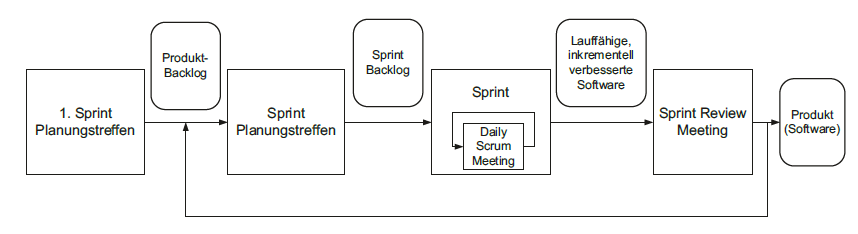
\includegraphics[width=8cm]{img/scrum.png}
			\caption{agiles Vorgehen: Scrum \autocite[372]{Alpar2019}}
			\label{img:scrum}
		\end{minipage}
	\end{figure}
	
	Der ein weiterer Ansatz des Projektmanagements ist das agile Vorgehen. Bei dem primär in der Softwareentwicklung genutzten Ansatz liegt das Augenmerk auf der Agilität, die durch das verbesserte eingehen auf den Kunden gewährleistet wird. Dadurch werden die einzelnen Phasen nicht genau durchgeplant, vielmehr wird eine iterative Vorgehensweise angestrebt, bei welcher der Kunde stets berücksichtigt wird. Ein Typisches Modell dafür ist \enquote{SCRUM}. Dieses Modell wird anhand von fest definierten Zeitabschnitten, welche \enquote{Sprints} genannt werden, abgearbeitet.\autocite[57-70]{Känel_2020_Projektphasen}\autocite[Kap. 1.3]{Alam2020}
	Die Abbildung \ref{img:scrum} beschreibt den Prozess der agilen Vorgehensweise Scrum.
	
	Bei der Umsetzung von Projekten in der Praxis ist eine solche saubere Abgrenzung zwischen der klassischen, sowie der agilen Vorgehensweise oft nicht möglich, daher gewinnen Kombinationen der beiden ersten Ansätze an Bedeutung. Diese hybriden Vorgehensweisen entnehmen einzelne Phasen oder Teilprojekte aus den entsprechenden Konzepten und kombinieren sie mit einem anderen  Ansatz. 
	So kann es beispielsweise sein, dass ein Softwareentwicklungsprojekt die Phasen der Projektdefinition, Anforderungsanalyse und Entwurf aus dem Wasserfallmodell entnehmen, die Implementierung und Integration jedoch agil gestaltet wird.\autocite[65]{Känel_2020_Projektphasen}
	
	Die genannten Ansätze unterscheiden sich zwar von der Vorgehensweise, zielen jedoch alle auf eine Strukturierung von Projekten ab, wodurch eine Wertsteigerung gewährleistet werden kann. Ein zentrales Werkzeug für die Sicherstellung der Qualität bei der Planung in Projekten ist der Projektstrukturplan. Durch ihn können den Phasen einzelne Arbeitspakete zugeordnet werden, die es abzuarbeiten gilt. 

\section{Projektstrukturplan}
	Der \ac{PSP} ist laut der DIN 69901-5 Norm eine \enquote{vollständige hierarchische
	Darstellung aller Elemente (Teilprojekte, Arbeitspakete) der Projektstruktur als
	Diagramm oder Liste}\autocite{DIN_Projektplan}
	Er fasst die unterschiedlichen Phasen zusammen und ordnet ihnen Aufgaben zu. Somit kann nicht nur der Fortschritt besser gemessen, sondern auch die Zuordnung der Verantwortlichkeiten im Projekt zugeteilt werden. 
	
	Aufgebaut wird der \acs{PSP} hierarchisch, die Hierarchie wird nach einem Top-Down bestimmt. Im Folgenden die hierarchische Gliederung des \acs{PSP}: 
	
	\begin{enumerate}
		\item \textbf{Projekt}
			\subitem Hier werden im \acs{PSP} sowohl die Ziele des gesamten Projektes dokumentiert als auch der Projektauftrag. 
			
		\item \textbf{Teilprojekte/ Projektphasen}
			\subitem Diese Phasen dienen der allgemeinen Übersicht über den Projektablauf. Jede Phase besitzt meistens einen Teilprojektleiter, der für die Fertigstellung seines Teils verantwortlich ist. 
		
		\item \textbf{Arbeitspakete}
			\subitem Arbeitspakete sorgen für eine klare Struktur der Aufgaben. Sie fassen eine bestimmte Zahl von Aufgaben zu einem Paket zusammen. Das Ziel ist eine eindeutige Zuordnung von Kosten, Ressourcen und Zeitaufwand zu schaffen. Die Namensgebung muss daher eindeutig gewählt werden, damit eine Abgrenzung möglich ist. Ein Arbeitspaket umfasst den Namen des verantwortlichen Bearbeiters, die Aufgabenbeschreibung, Abnahmebedingungen, den Bearbeitungsaufwand sowie den Ressourcenbedarf. 
		
		\item \textbf{Aufgaben}
			\subitem Sind die kleinste Einheit in einem Projekt. Sie beschreiben die zu erbringende Tätigkeit in dem Arbeitspaket. 
		
	\end{enumerate}

	Neben der hierarchischen Aufteilung besitzt der \ac{PSP} mehrere Möglichkeiten einer Gliederung. 
	
	\begin{itemize}
		\item Verrichtungsorientiert
			\subitem Aufgaben die erfüllt sein müssen, damit das Projekt verwirklicht wird.
		
		\item Objektorientierung
			\subitem Plant Ergebnisse sowie Lieferobjekte die im Laufe der Phase/ Projektes zu erledigen sind. 
		
		\item Phasenorientierung
			\subitem Orientiert sich an den Phasen aus dem Projektmanagement
	\end{itemize} 

	Wegen der Komplexität heutiger Projekte, sowie deren mehrdimensionaler Projektstruktur kommt es nicht selten zu einer Mischform dieser Gliederungsarten. \autocite[387-391]{Alpar2019}

\section{Arbeitspakete}
\label{sec:arbeitspakete}

	Unter einem \ac{AP} wird die Beschreibung der Aufgabe im Prozess bezeichnet, die von einer Person bzw. einer Abteilung in der festgelegten Zeit zu mit dem vereinbarten Aufwand zu vollbringen ist.\autocite[196]{Känel_2020_Projektphasen} In einem Arbeitspaket werden daher unterschiedliche Informationen festgehalten, die einem Projektmanager helfen eine Planung durchzuführen. Es wird neben der Beschreibung auch eine eindeutige Nummer, die Start und Ende Zeit, die Kosten, der Ressourcenbedarf etc. festgelegt. Die \autoref{img:arbeitspaket} zeigt ein beispielhaftes Layout. 
	
	\begin{figure}[h]
		\centering
		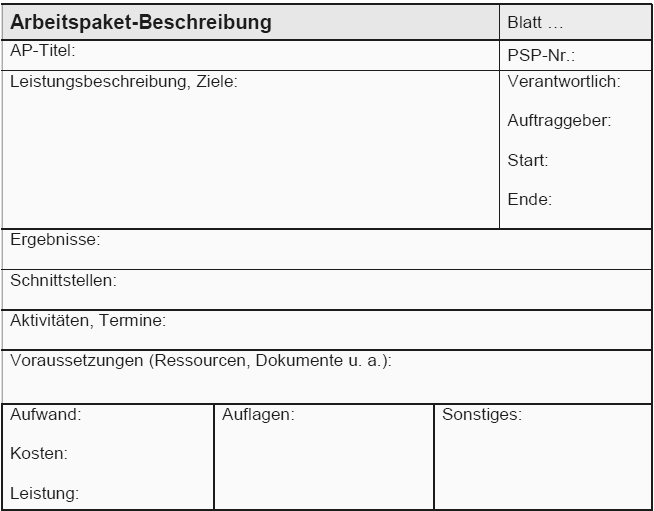
\includegraphics[width=15cm]{img/Arbeitspacket.png}
		\caption{Phasen der unterschiedlichen Normen\autocite[170]{Känel_2020_Projektphasen}}
		\label{img:arbeitspaket}
	\end{figure}
	
	
	
	
	
	
	
	
	
	
	
	
	